%20 min preso!
\documentclass[xcolor=table]{beamer}
\usepackage{beamerthemesplit}
\usepackage{wrapfig}
\usetheme{SPBU}
\usepackage{pdfpages}
\usepackage{amsmath}
\usepackage{cmap}
\usepackage[T2A]{fontenc}
\usepackage[utf8]{inputenc}
% \usepackage[english]{babel}
% \usepackage[russian]{babel}
\usepackage{indentfirst}
\usepackage{amsmath}
\usepackage{tikz}
\usepackage{multirow}
\usepackage[noend]{algpseudocode}
\usepackage{algorithm}
\usepackage{algorithmicx}
\usepackage{fancyvrb}

\usepackage{caption}
\usepackage{subcaption}

\usetikzlibrary{calc}
\usetikzlibrary{shapes,arrows}
\usetikzlibrary{arrows,automata}
\usetikzlibrary{positioning}

\usepackage{hyperref}
\hypersetup{
    colorlinks=true,
    linkcolor=blue,
    filecolor=magenta,      
    urlcolor=cyan,
}

%usepackage{fancyvrb}
%\usepackage{minted}
%\usepackage{verbments}
\usepackage{fontawesome}

%for [[]]
\usepackage{stmaryrd}

\usepackage{caption}

%code highlight
\usepackage{listings}
\usepackage{xcolor}
 
\definecolor{codegreen}{rgb}{0,0.6,0}
\definecolor{codegray}{rgb}{0.5,0.5,0.5}
\definecolor{codepurple}{rgb}{0.58,0,0.82}
\definecolor{backcolour}{rgb}{0.95,0.95,0.92}
 
\lstdefinestyle{mystyle}{
    backgroundcolor=\color{backcolour},   
    commentstyle=\color{codegreen},
    keywordstyle=\color{magenta},
    numberstyle=\tiny\color{codegray},
    stringstyle=\color{codepurple},
    basicstyle=\ttfamily\footnotesize,
    breakatwhitespace=false,         
    breaklines=true,                 
    captionpos=b,                    
    keepspaces=true,                 
    numbers=left,                    
    numbersep=5pt,                  
    showspaces=false,                
    showstringspaces=false,
    showtabs=false,                  
    tabsize=2
}
 
\lstset{style=mystyle}

\usepackage{tabularx}
\newcolumntype{Y}{>{\raggedleft\arraybackslash}X}

\renewcommand{\thealgorithm}{}

\newtheorem{mytheorem}{Theorem}
\renewcommand{\thealgorithm}{}

\newcommand{\tikzmark}[1]{\tikz[overlay,remember picture] \node (#1) {};}
\def\Put(#1,#2)#3{\leavevmode\makebox(0,0){\put(#1,#2){#3}}}

\newcommand{\ltz}{$< 1$}


\tikzset{
    state/.style={
           rectangle,
           rounded corners,
           draw=black, very thick,
           minimum height=2em,
           inner sep=2pt,
           text centered,
           },
}

\beamertemplatenavigationsymbolsempty

\title[Реализация и применение алгоритмов]{\large{Реализация и применение строковых алгоритмов к задаче поиска повторов в документации программного обеспечения}}
% subtitle[YaccConstructor]{Parsing techniques for graph analysis}
% То, что в квадратных скобках, отображается в левом нижнем углу.
\institute[СПбГУ]{
Санкт-Петербургский государственный университет \\
Кафедра системного программирования }

% То, что в квадратных скобках, отображается в левом нижнем углу.
\author[Никита Мишин]{\scriptsize{{\bfseries Автор:} Мишин Никита Матвеевич, группа 16.Б11-мм}\\ \vfill
  \and  
    {\scriptsize{\bfseries Научный руководитель:} к.ф-м.н., доцент С.\,В.\,Григорьев}\\
	\and
	{\scriptsize{\bfseries Научный консультант:} к.ф-м.н. Д.\,А.\,Березун}\\
	\and
	{\scriptsize{\bfseries Рецензент:} д.\,ф.\,н., Тискин А.\,В.}
	}

\date{13 июня 2020г.}

\begin{document}
{
\begin{frame}[fragile]
  \begin{tabular}{p{2.0cm} p{7.5cm} p{1cm}}
   \begin{center}
    \end{center}
    &
    \begin{center}
    
\includegraphics[height=1.5cm]{pictures/SPbGU_Logo.png}
    \end{center}
    &
    \begin{flushright}
    \end{flushright}
  \end{tabular}
  \titlepage
  \thispagestyle{empty}
\end{frame}
}


% Введение 1 2 слайда
\begin{frame}{ Поиск повторов в документации ПО}
    Поиск повторяющихся фрагментов текста с целью:
    \begin{itemize}
    % \vfill\item Унификация документации
    \vfill\item Избавление от нежелательной избыточности
    \vfill\item Выявление ошибок и несогласованности
    \vfill\item Переиспользование повторяющихся фрагментов

    \vfill\item ...
    \end{itemize}
\end{frame}


\begin{frame}{Задачи поиска повторов}
\begin{itemize}
    \vfill\item Поиск шаблона в заданном тексте:
     \begin{flushright} Луцив Д. В. \emph{Поиск неточных повторов в документации программного обеспечения} (диссертация, 2018)  
    \end{flushright}
    \vfill\item Поиск групп повторов:
    \begin{itemize}
        \vfill\item Неясно, насколько часто встречаются древовидные группы повторы
        \vfill\item Часто ищут в \emph{JavaDoc} документации
    \end{itemize}
\end{itemize}
\end{frame}



\begin{frame}{semi-local LCS и SA}
    \begin{itemize}
        \vfill\item Позволяет решать более широкий класс задач:\\
        % \hfill 
        \begin{flushright}
         Tiskin A. \emph{Semi-local string comparison: algorithmic techniques and applications (draft-book)} 
        \end{flushright}
        \vfill\item Алгоритмы с хорошими теоретическими показателями
        \vfill\item Не применялись к поиску к поиску повторов в документации
        \vfill\item Не были реализованы на практике
        
    \end{itemize}

    
\end{frame}


\begin{frame}{Постановка задачи}
    Цель:
    \begin{itemize}
        \vfill \item \emph{Адаптация алгоритмов решения задач полулокальных поиска наибольшей общей подпоследовательности и выравнивая строк к задачам поиска повторов в  документации ПО}
    \end{itemize}
    \vfill Задачи:
    \begin{enumerate}
    \vfill\item  Исследовать существующие теоретические алгоритмы решения задач полулокального поиска наибольшей общей подпоследовательности и выравнивания строк и реализовать их на практике в виде \emph{библиотеки алгоритмов}
    \vfill\item Адаптировать алгоритмы решения полулокальных задач  поиска \emph{LCS} и \emph{SA} к задаче поиска повторов в \emph{JavaDoc} документации и реализовать соответствующее приложение на их основе
    \vfill\item Провести экспериментальное исследование реализованных алгоритмов  и анализ результатов
    \end{enumerate}
\end{frame}



\begin{frame}{Библиотека алгоритмов \emph{semi-local} задач: Алгоритмы}
\begin{itemize}
    \vfill\item Необходимые структуры данных
    \vfill\item Алгоритмы для решения semi-local \emph{LCS} и \emph{SA}:
    \begin{enumerate}
        \vfill\item Распутывание кос
        \vfill\item Матричное умножение через тропическую алгебру
        \vfill\item Умножение кос
    \end{enumerate}
    \vfill\item Алгоритмы, решающие задачи на основе \emph{semi-local}:
    \begin{enumerate}
        \vfill\item Window-substring
        \vfill\item Поиск шаблона в тексте
        \vfill\item Локальное выравнивание с ограничениями:
        \begin{flushright}
            Tiskin A. \emph{Bounded-Length Smith-Waterman Alignment} (WABI 2019) 
    \end{flushright}
    \vfill\item ...
    \end{enumerate}
\end{itemize}
\end{frame}



\begin{frame}{Алгоритмы поиска дубликатов}
\begin{itemize}
    \item Поиск по шаблону
    \begin{enumerate}
        \vfill\item Улучшенная асимптотическая версия алгоритма из диссертации
        \vfill\item Алгоритмы на основе анализа решения \emph{semi-local}
    \end{enumerate}
    \vfill\item Поиск групп повторов в \emph{JavaDoc}
    \begin{enumerate}
        \vfill \item Графовые алгоритмы с матрицей расстояний на основе \emph{semi-local} и её производных 
        %  сказать про лики
    \end{enumerate}
\end{itemize}
    
\end{frame}


\begin{frame}{Приложение для поиска повторов в \emph{JavaDoc}}
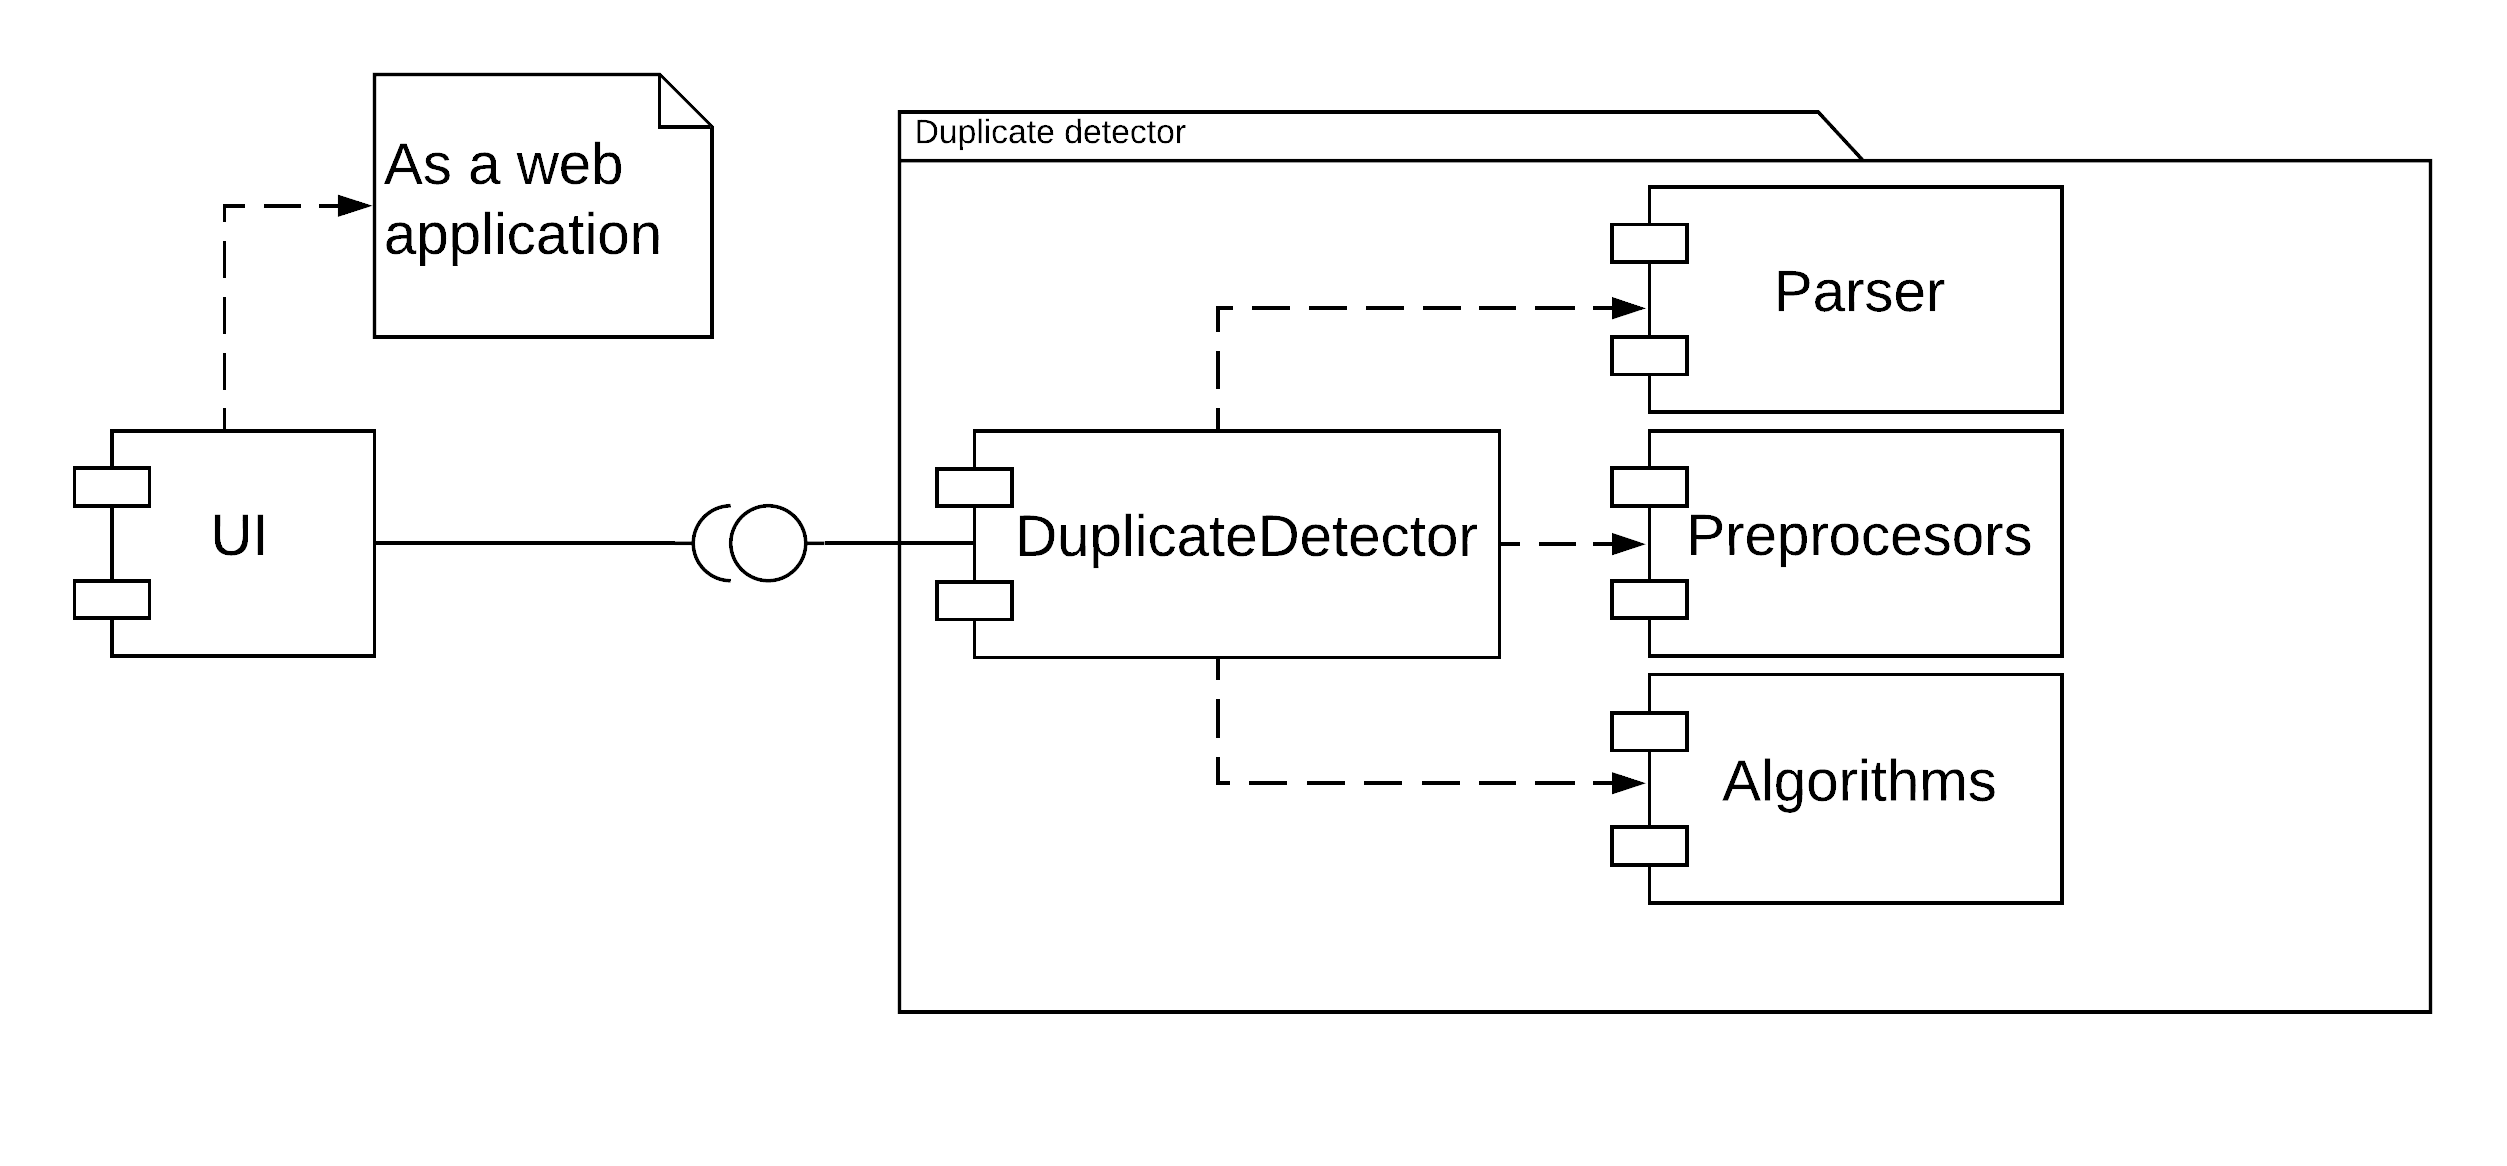
\includegraphics[width=1.0\textwidth]{pictures/arhitecture.png}
\end{frame}




\begin{frame}{Визуализатор}

\begin{figure}
    \centering
 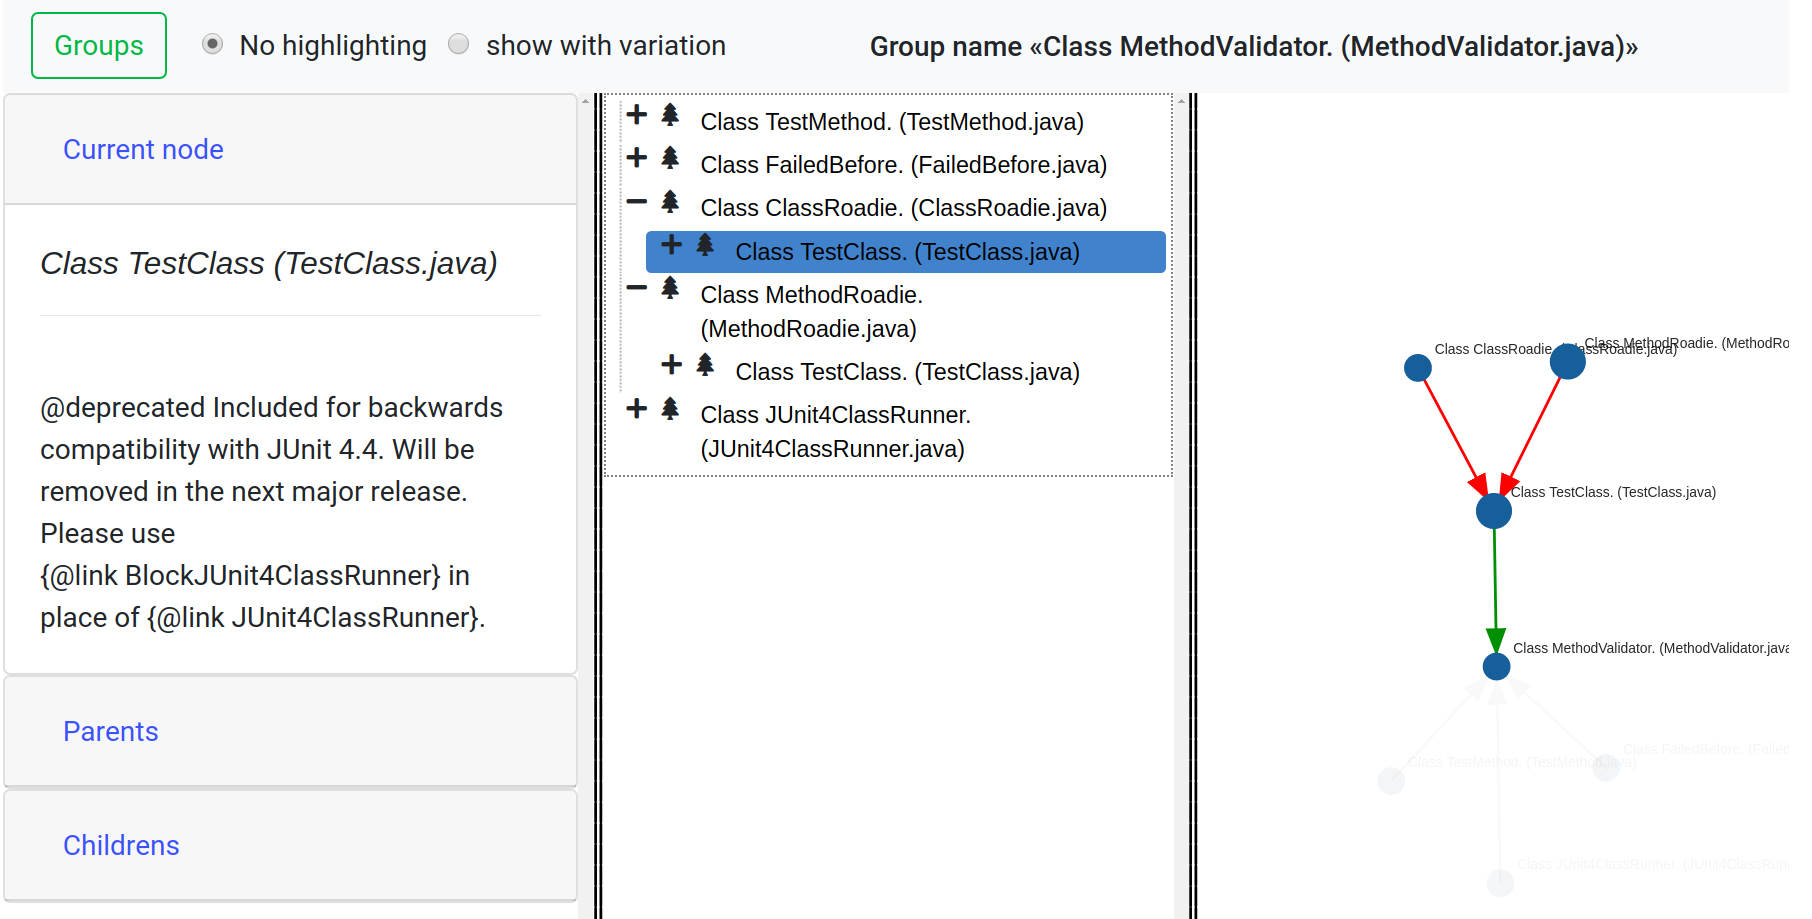
\includegraphics[width=1.0\textwidth]{pictures/exampleViz.png}
 \caption{Пример визуализации для группы повторов}
 \end{figure}
\end{frame}


\begin{frame}{Апробация: Применимость на практике алгоритмов решения задач \emph{semi-local}}

\begin{figure}
    \centering
    \begin{subfigure}[b]{0.45\textwidth}
    \centering
    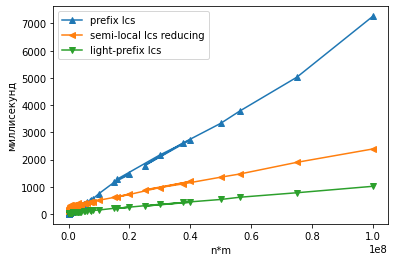
\includegraphics[width=\textwidth]{pictures/semiLocalvsPrefixLCS.png} \caption{semi-local lcs vs prefix lcs}
    \label{fig:subim1}
    \end{subfigure}%
    % \hfill
    \begin{subfigure}[b]{0.45\textwidth}
    \centering
    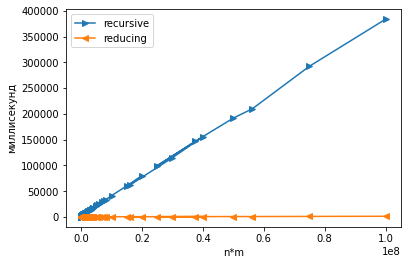
\includegraphics[width=\textwidth]{pictures/semilocalReducignVssemiLocalRecursive.png}
    \caption{recursive vs reducing approach}
    \label{fig:subim2}
    \end{subfigure}
\caption{Сравнение скорости реализаций, решающих полулокальные задачи}
\end{figure}


\end{frame}


\begin{frame}{Апробация: Применимость \emph{semi-local} к задаче  поиска по шаблону}
\begin{figure}
    \centering
    \begin{subfigure}[b]{0.45\textwidth}
    \centering
    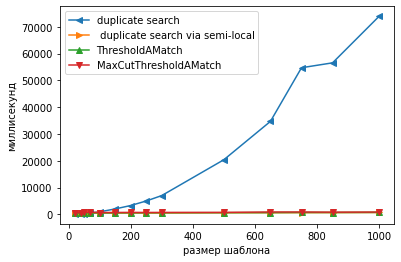
\includegraphics[width=\textwidth]{pictures/smallAlphabet.png} \caption{Сценарий с малым размером\\ алфавита}
    \label{fig:subim1}
    \end{subfigure}%
    % \hfill
    \begin{subfigure}[b]{0.45\textwidth}
    \centering
    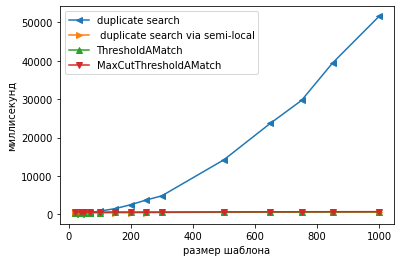
\includegraphics[width=\textwidth]{pictures/largeAlphabet.png}
    \caption{Сценарий с большим размером\\ алфавита}
    \label{fig:subim2}
    \end{subfigure}
\caption{Сравнение скорости различных алгоритмов решения задачи \emph{поиска по шаблону}}\label{ssss}
\end{figure}

\end{frame}

% \begin{frame}{Апробация: Применимость \emph{semi-local} к задаче  поиска групп повторов}
% \begin{itemize}
%     \vfill\item Алгоритмы на основе решения задач \emph{semi-local} могут быть успешно применены к задаче \emph{поиска групп повторов}
%     \vfill\item Группы преимущественно состоят из одинаковых фрагментов (одинаковые методы, схожая функциональность) с незначительными изменениями (в графе это клики)
%     \begin{itemize}
    
%         \vfill\item Сложная структура дерева (без учета клик) практически не присутствует
%     \end{itemize}
%     \vfill\item Количество повторов в \emph{JavaDoc}-документации существенно, что подтверждает результаты из статей
%     \vfill\item Построение полного графа похожести --- долгая операция
%     \begin{itemize}
%         \vfill\item Нужен предпроцессинг для сокращения количества ребер
%     \end{itemize}
% \end{itemize}
% \end{frame}

\begin{frame}{Апробация: Применимость \emph{semi-local} к задаче поиска групп повторов}
    \begin{figure}
\begin{center}
 \begin{tabular}{ | p{2cm} | p{2cm} | p{2cm} | p{2cm} | p{2cm} |} 
 \hline
 
 Название  проекта & Кол-во  комментариев & Кол-во  повторов & Кол-во групп & Время исполнения (сек) \\
 \hline
  slf4j & 188 & 157 & 25 & 8 \\
  \hline
  apache commons io & 1284 & 1180 & 92 & 569 \\
  \hline
  apache commons collection & 610 &495 &50 & 408 \\
  \hline
  gson & 498 & 356 & 81 & 96 \\
  \hline junit & 680 & 539 & 87 & 163 \\
  \hline mockito & 2979 & 2812 & 164 & 2012\\
  \hline guava & 4340 & 3662 & 418 & 8505 \\
  \hline
\end{tabular}
\end{center}
\caption{Результат работы приложения}\label{table}
\end{figure}
\end{frame}

\begin{frame}{Апробация: Применимость \emph{semi-local} к задаче поиска групп повторов}

\begin{figure}
    \centering
 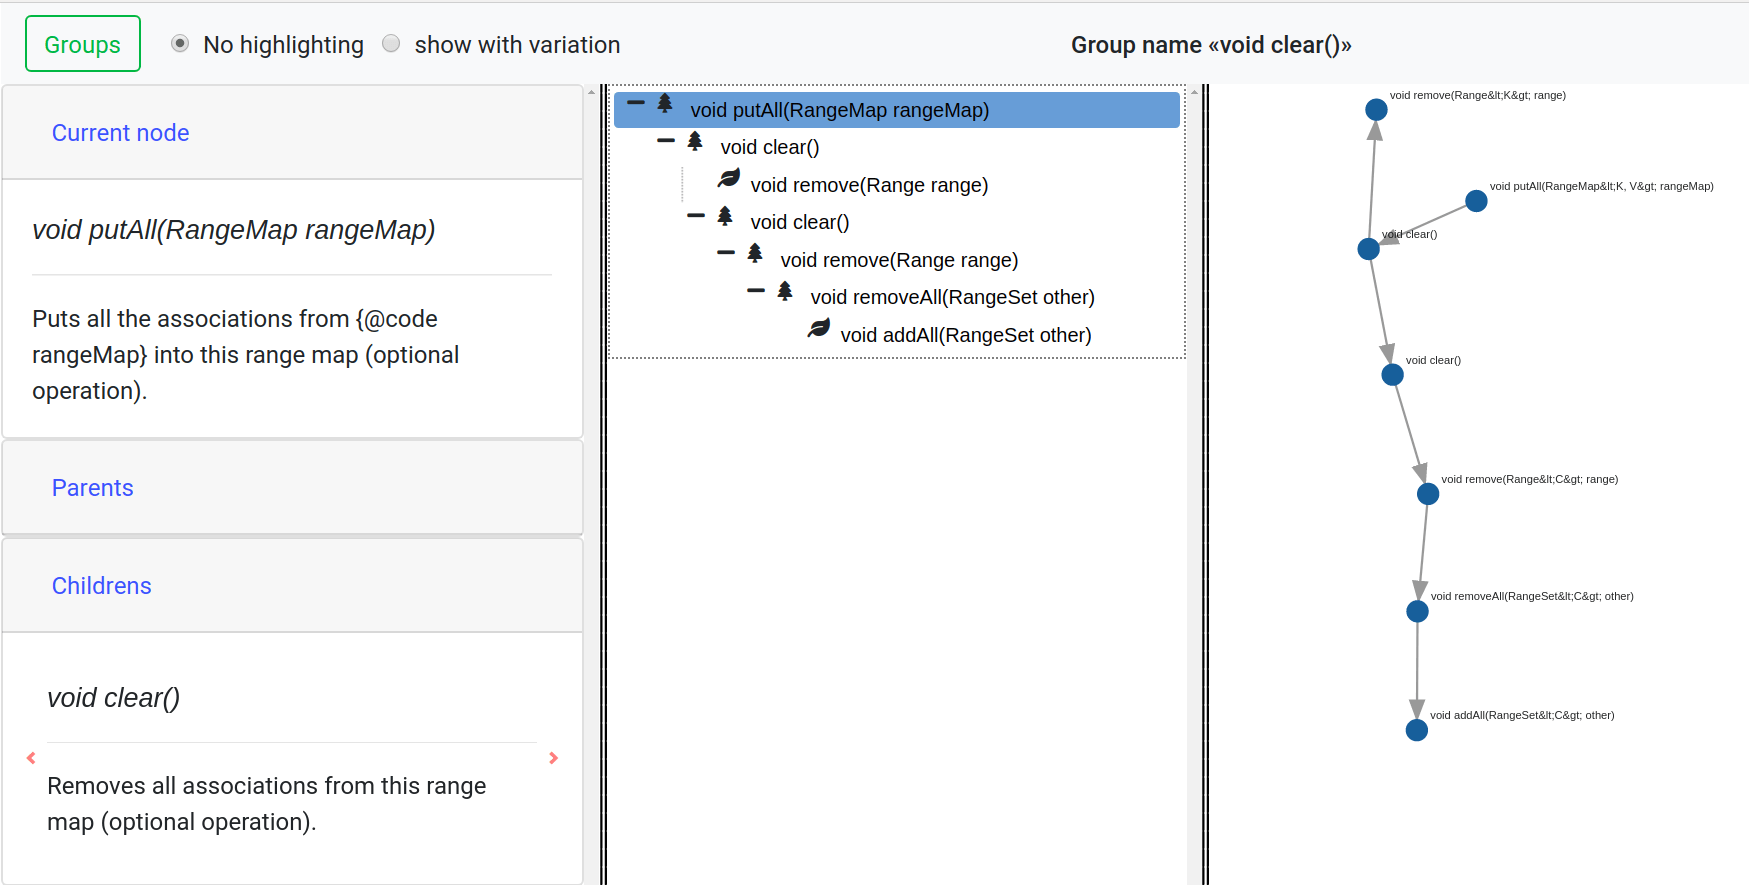
\includegraphics[width=1.0\textwidth]{pictures/outputGroup.png}
 \caption{Пример группы из проекта \emph{guava}}
 \end{figure}
\end{frame}


\begin{frame}{Результаты}
    \begin{itemize}
    \vfill\item Исследованы существующие теоретические алгоритмы решения задачи полулокального поиска наибольшей общей подпоследовательности и  выравнивания строк и реализованы в виде     \emph{библиотеки алгоритмов} на языке \emph{Kotlin}
    \vfill\item Создано приложение на языке \emph{Kotlin} для поиска повторов в \emph{JavaDoc} документации на основе адаптации алгоритмов решения полулокальных задач
    \vfill\item Проведено экспериментальное исследование реализованных алгоритмов  и  анализ результатов
    \end{itemize}
       
\end{frame}




\end{document}